\documentclass[twocolumn]{article}
% Bibliography used for citing
\usepackage[backend=biber,
	bibencoding=utf8,
	style=numeric-comp
]{biblatex}
\addbibresource{bib/mybib.bib}
\addbibresource{bibliography.bib}
\usepackage{amsmath}
\usepackage{amsfonts}
\usepackage{semantic}
\usepackage{mathrsfs}
\usepackage{tabularx}
\usepackage{booktabs}
\usepackage{hyperref}
\usepackage{cleveref}
\usepackage{listings}
\usepackage{todonotes}
\usepackage{color}
\usepackage{algorithm}
\usepackage{algpseudocode}
\usepackage{mathtools}
\usepackage{amsmath}
\definecolor{light-gray}{gray}{0.85}
\lstset{
	numbers=left,
	breaklines=true,
	backgroundcolor=\color{light-gray},
	tabsize=2,
	basicstyle=\ttfamily,
	literate={\ \ }{{\ }}1
}
\crefname{equation}{}{}
\mathlig{-><-}{\rightarrow\leftarrow}
\newcommand{\sep}{\:|\:}
\newcommand{\oracle}{\ensuremath{\mathscr{I}}}
\newcommand{\staticlang}{\ensuremath{\mathscr{L}_s}}
\newcommand{\dynlang}{\ensuremath{\mathscr{L} \:}}
\newcommand{\aware}{\ensuremath{A_a\varphi}}
\newcommand{\know}{\ensuremath{K_a\varphi}}
\newcommand{\anso}{\ensuremath{R_{\Phi}}}
\newcommand{\ansa}{\ensuremath{R_{a}}}
\newcommand{\powset}{\ensuremath{\mathscr{P}}}
\newcommand{\oset}{\ensuremath{((\gamma_1,...,\gamma_k), \gamma_i)}}
\newcommand{\aset}{\ensuremath{((\varphi_1,...,\varphi_n), \varphi_j)}}
\newcommand{\proposition}{\ensuremath{\varphi\:}}
\newcommand{\dilmodel}{\ensuremath{\langle W, \sim_{a\in Ag}, V, A_{a\in Ag}, \Phi, R_{\Phi, a\in Ag}\rangle}}
\newcommand{\pubop}{\ensuremath{\left[\psi!\right]\varphi}}
\newcommand{\agquestop}{\ensuremath{\left[(\varphi_1,...,\varphi_n)?\right]_{a,b} \varphi}}
\newcommand{\infop}{\ensuremath{\left[\{\psi_1,...,\psi_m \}\hookrightarrow
			\psi_c\right]_a \varphi}}
\usepackage{graphicx}
\usepackage[font=scriptsize, skip=-2pt]{caption}
\usepackage{float}
\usepackage{graphicx}

\begin{document}
\title{Title}
\author{
	Hugin Juliansson Zachariasen \\ Aalborg University \\ hjulia21@student.aau.dk
	\and
	Kristian Hadberg Mikkelsen \\ Aalborg University \\ khmi22@student.aau.dk
	\and
	Lucas Mørk Frendorf \\ Aalborg University \\ lfrend21@student.aau.dk
	\and
	Nicklas Peter Kvist Gislinge \\ Aalborg University \\ ngisli21@student.aau.dk
}
\maketitle
\begin{abstract}
	Abstract goes here.
\end{abstract}

\section{Introduction}
When trying to solve a problem, many solutions may present themselves. However,
most of these will come with unintended side effects. In the world of social
deduction games, one specific problem has manifested itself. As more diverse
roles has been introduced, in order to keep the games fresh, new, and exciting,
an imbalance has presented itself in the win-rate between the opposing teams.
\\ \\ Most social deduction games have the same foundation: The players are
divided into two teams, one larger with uninformed players, and one smaller
with informed players. Each of the teams wants to eliminate the other team,
with differing methods of accomplishing this. Often, the uninformed team will
have a few special roles assigned to it, in order to be able to acquire
information, to be able to root out the smaller team. The smaller team
typically tries to stay hidden, while eliminating the players in the bigger
team.\\ \\ Historically, the larger team has typically been burdened by the
assignment of many low-impact roles to its players. As games have evolved,
players have grown bored with this dynamic and that has led to the introduction
of more roles, in order to excite the players who were previously assigned the
low-impact roles. But as their roles are no longer low-impact, this has skewed
the win-rate of their team in their favour. This is problematic from a balance
perspective, and therefore this paper will look at how one can analyse and
introduce roles to the opposing team, in order to equalize this imbalance. The
roles that will be analysed consist mainly of two types: information- gatherers
and deniers. Through this analysis we will be able to draw a general conclusion
on the topic of whether it is more important to gather information for your own
benefit, or to deny information to opposing entities.

This will be analysed by utilizing a self-developed, console-based simulation
of a social deduction game, incorporating a numeric approach to
decision-making, with a foundation in epistemic logic. The game will be
modelled with a variety of roles and actions, as well as voting strategies and
communicative actions.

A sizeable amount of research has been put into the field of social deduction
games. However, much of that research has been focused on strategies relating
to when and how to utilize different communicative actions\cite{commitment}.
Some focus on ways for the town to detect the mafia
members\cite{werewolf_stealth}, or protect key town members from the
mafia\cite{werewolf_nash_equilibrium}. Others focus on the different
decision-making strategies that can be implemented in multiagent systems, which
these games can be modelled
as\cite{modelling_multi_agent_epistemic_systems}\cite{multi_agent_epistemic_planner_common_knowledge}\cite{probibalistic_multiagent_systems}.

However, one thing that is noticeably absent from this research is analyses
with the focus of mitigating the previously mentioned side effect, that arises
when playing against a team consisting of mostly high-impact roles.
Additionally, there is minimal research on the ability to inquire other
players, regarding their knowledge of the world. The outcome of such an
analysis might be a game setup where everyone involved can have a role with
special abilities. This may also mean that players will be more engaged and
active throughout all stages of the game. Lastly, it may also grant some
insight into whether it is more beneficial to gather information for oneself,
or to deny information to others.\\ \\

In the following section \ref{sec:RelatedWorks}, we will review papers and
studies that have significantly contributed to our work.

We then describe how we intend to model our social deduction game in section
\ref{sec:Modelling}. It outlines the rules of the game and its operational
mechanics. Key roles will be explained in detail, as well as how agents
communicate with each other. Furthermore, we will explain our 'mark' system and
'world elimination' in this section.

Moving over to the dynamic inquire language section
\ref{sec:DynamicInquiryLanguage}. This section begins with an introduction to
the terminology and the inquiry language. We then expand this to a static
inquiry language with agents and knowledge. Finally, we conclude the section by
expanding it to a dynamic inquiry language with model updates.

For the implementation section \ref{sec:implementation}, we provide a detailed
walkthrough of all the processes utilized in our implementation. We start by
introducing the various data structures and then explain how each 'phase' of
the game is computed. \todo{Adjust to follow the new format when section 5 is
    updated}

In the final sections of the paper \ref{sec:results}, \ref{sec:discussion}, and
\ref{sec:conclusion}, we present all our findings from our experiments.
\section{Related Works}
A sizable amount of research has been put into the field of social deduction 
games. However, much of that research has been focused on strategies relating 
to when and how to utilize different communicative actions\cite{commitment}. 
Others focus on ways for the town to detect the mafia 
members\cite{werewolfstealth}, or protect key town members from the 
mafia\cite{werewolfnashequilibrium}, and others still focus on the different 
decision making strategies that can be implemented in multi agent systems, 
which these games can be modeled 
as\cite{modellingmultiagentepistemicsystems}\cite{multiagentepistemicplannercommonknowledge}\cite{probibalisticmultiagentsystems}.
 However, one thing that is noticeably absent from this research is analyses 
with the focus of "evening the odds" for the mafia team when faced with a town 
full of special roles. The outcome of such an analyses might be a game setup 
where everyone involved can have a role with special abilities, meaning that 
players will likely be more engaged and active, throughout all stages of the 
game. 

In a paper [1], Eger and Martens analyzed the effect of commitment to a plan in
the game One Night Ultimate Werewolf. They modeled this using Dynamic Epistemic
Logic, allowing each agent to be aware of multiple different possible worlds
with alternating sets of facts, and sorting them based on the least likelihood
of it being true. This is achieved by ‘marking’ worlds with statements made by
other agents if these worlds contained lies made by the other agents. When an
agent needs to choose what to base their next action on, they determine based
on the number of marks of other players, or simply nothing. They proclaim this
gives the agents a certain degree of planning. However, due to the increasing
amount of worlds generated by new actions performed, many of them equivalent, a
notion of commitment is introduced, in which they will stick with a certain
plan until another plan is valued significantly higher. They compare this
commitment to a baseline of random actions by villagers, resulting in a high
win percentage for werewolves, proving their hypothesis. In a game of both
werewolves and villagers with weighted worlds, they found that simply valuing
the plans equally, that is choose the new plan if it is at least as good as the
previous, resulted in the lowest win percentage for werewolves. The
Interrogative Model of Inquiry (IMI) and Dynamic Epistemic Logics (DEL) are
both central paradigms of formal epistemology, but where one lacks, the other
excels. While IMI provides knowledge reasoning and inference in a multi-turn
information-gathering process between an Inquirer and Nature, DEL models how
each agent updates their knowledge in a multi-agent setting. In 2014
Y.Hamami[2] published a formalization of how to combine these, which combines
the information-gathering process in an inquiry with respect to multi-agent
dimensions. As opposed to standard IMI or DEL, the proposed DELIMI sees
information as acquired by either common knowledge or from other agents in an
interrogation. The inclusion of agents also introduces the notion of lying,
that is answering an interrogative question with non-factual information,
closely representing the nature of social deduction games. In reality, both the
intrigue and the complexity of social deduction games often arise from the
discussions involved between players, which we see as a core part of this type
of game. While other works related to social deduction games have resorted
mostly to rely on simple one-way actions, the DELIMI model allows agents to
interrogate others, perhaps challenge their claims, find inconsistencies, or
use logical inference to establish presuppositions.

This work draws upon the foundational contributions of both Hintikka
!!Language, Truth and Logic in Mathematics!! and Kripke in establishing the
principles for reasoning about knowledge and belief. Specifically, we utilize
independence-friendly first-order logic. Additionally, we adopt the semantic
framework proposed by Baltag, Moss, and Solecki (2004) !!Logics for Epistemic
Actions: Completeness, Decidability, Expressivity!! to model the dynamic
aspects of knowledge and belief within different environments.

This work draws inspiration from prior research investigating imperfect
information games !!The epistemic logic of IF games!!, player strategies in
social deduction contexts !!Human-Side Strategies in the Werewolf Game Against
the Stealth Werewolf Strategy!!, and game-theoretic analysis !!Application and
Commercial Extension of Game Theory in Strategy games!!.s
\section{Modelling}
As mentioned earlier, we wish to model a framework of games instead of one
specific one, in order to encapsulate as many parameters as possible. The
simulation will have two factions, henceforth known as the town and the mafia.
The town wins when they have eliminated all mafia members. The mafia wins when
their factions have the non-strict numerical majority of players. The game is
played out in rounds consisting of four phases, which happen in order, until
either win-condition is met, as shown on figure \ref{fig:GameOverview}.
\begin{figure}[H]
	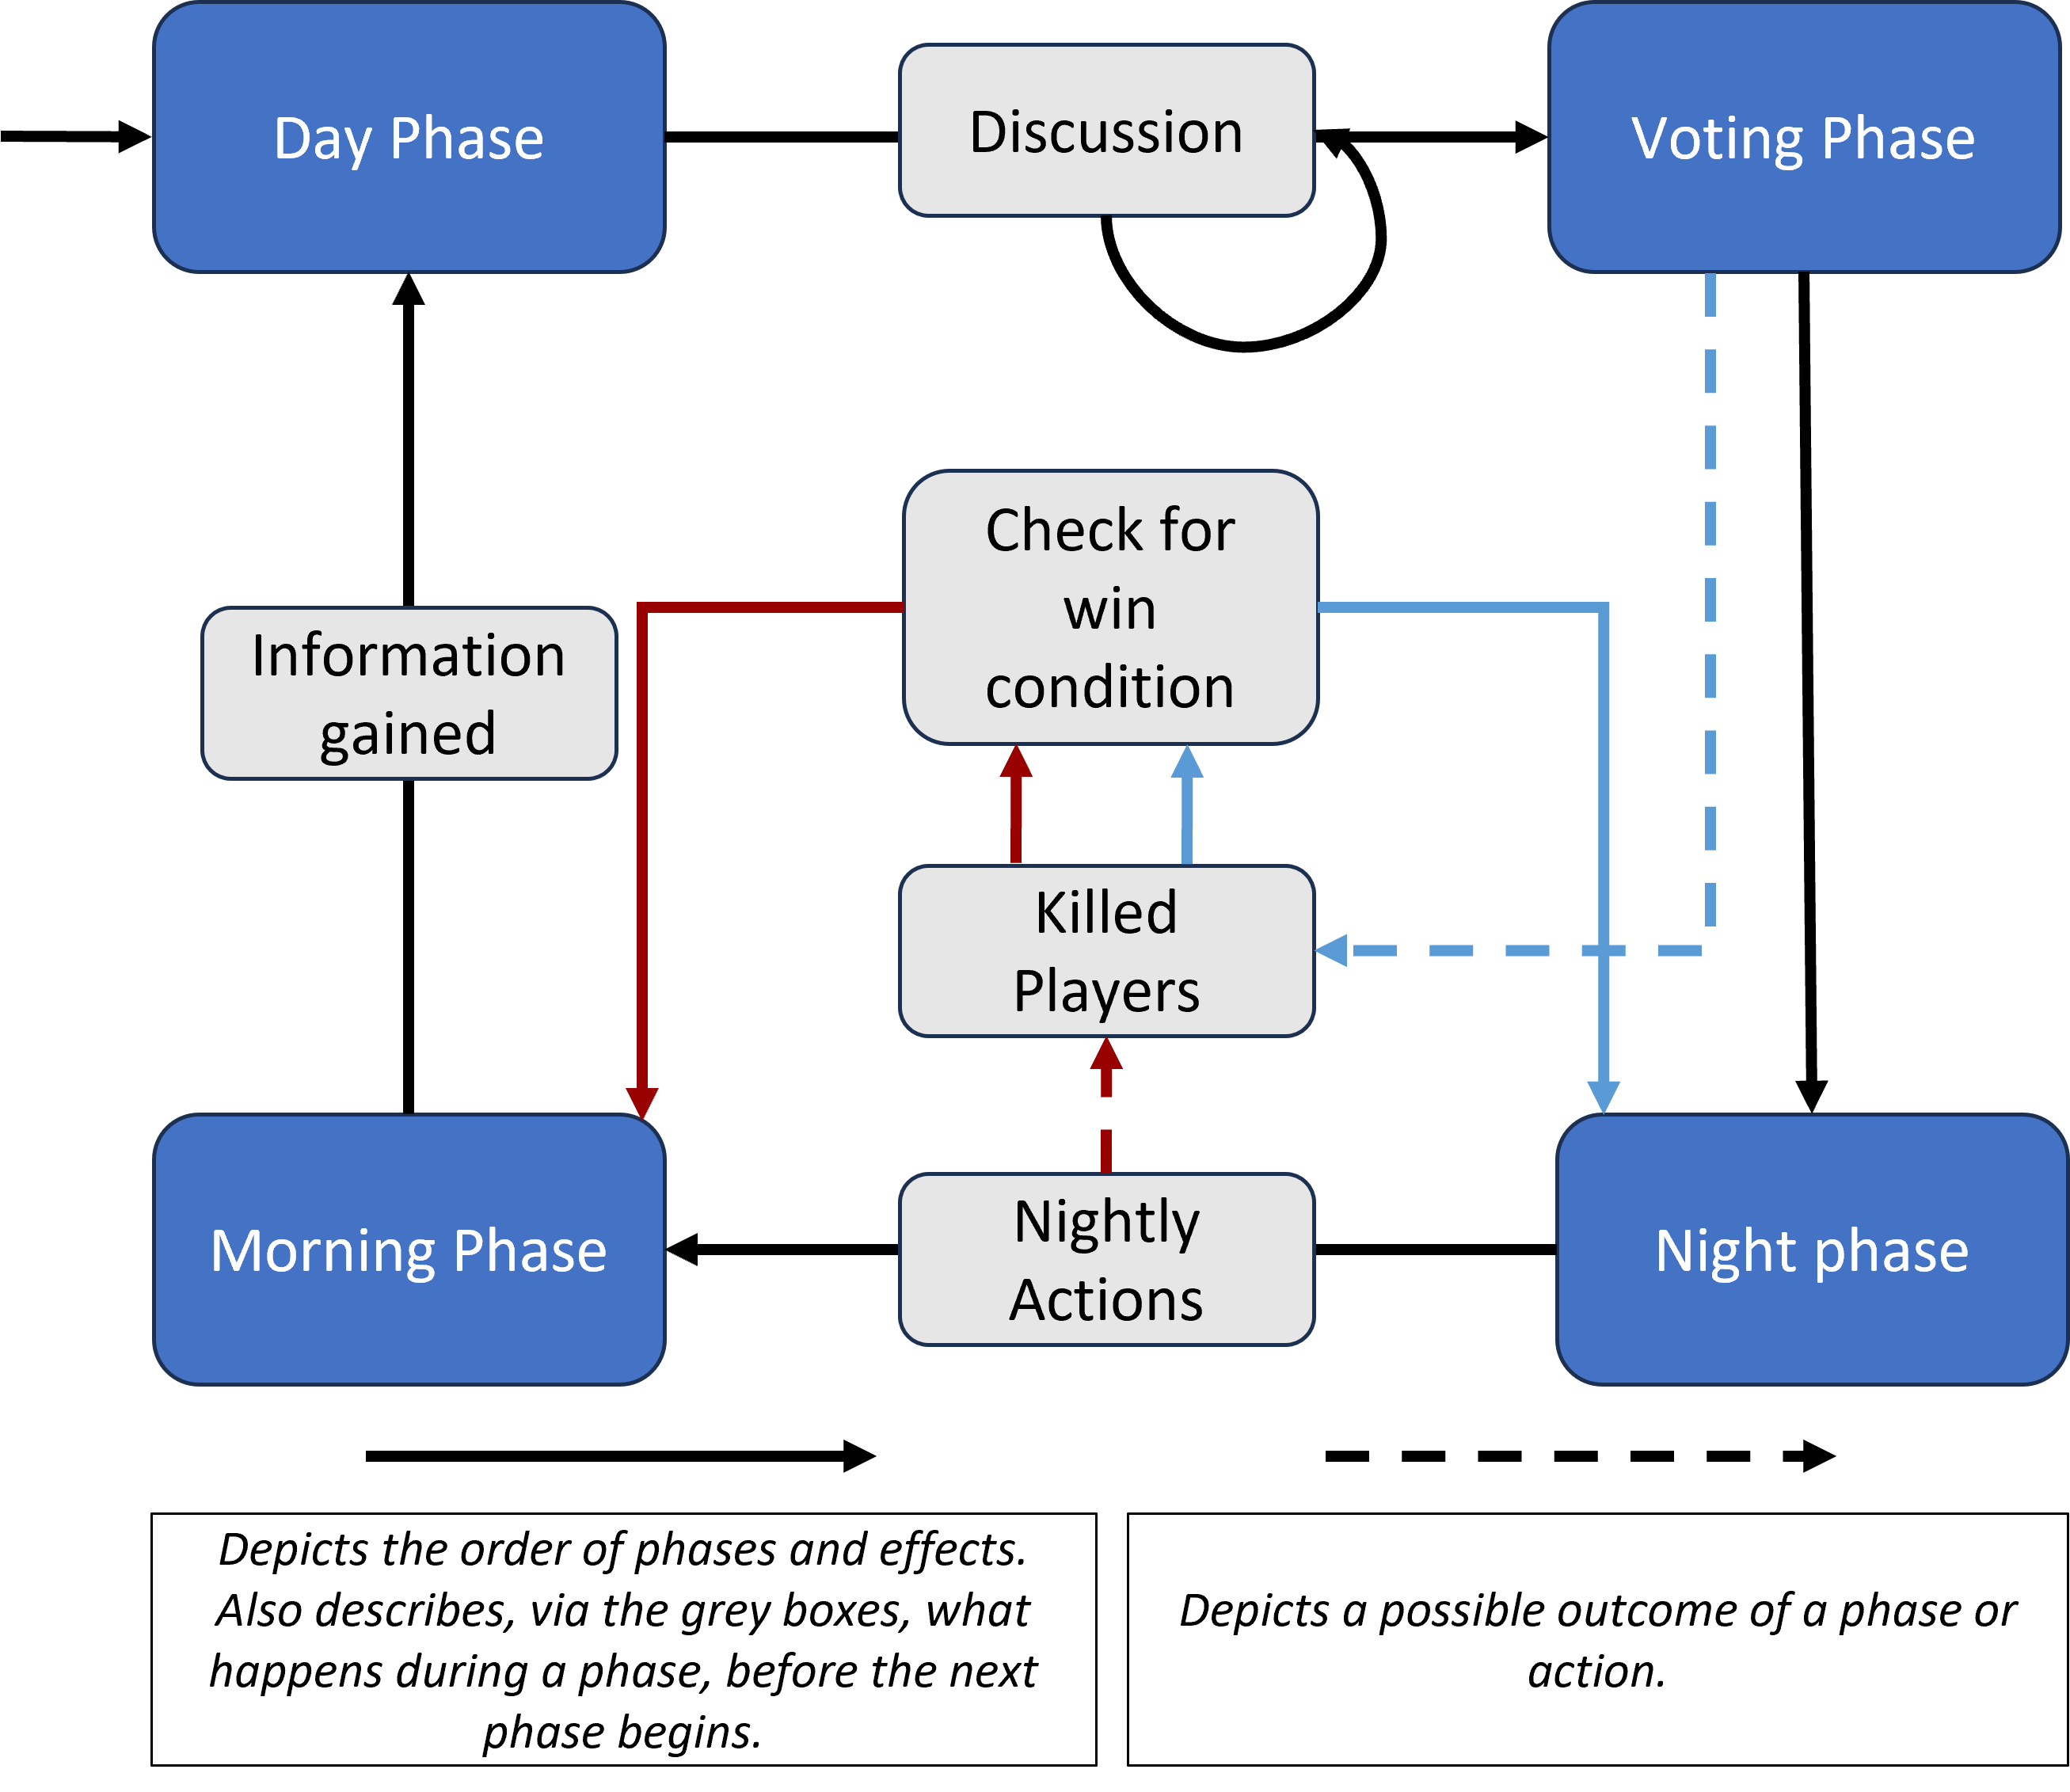
\includegraphics[width=1\linewidth]{figures/Game_overview}
	\caption{Depicting the general flow of social deduction games.}
	\label{fig:GameOverview}
\end{figure}

The night phase is where different roles perform private or public actions to
gain information or spread misinformation. The morning phase is where public
results of the night phase are revealed to all players. The roles of players
who died during the night phase is revealed at this time. The day phase is
where players try to influence each other's world views through communicative
actions. The voting phase is where players vote on who to lynch according to
their individual world views. The voting phase can end in a majority vote which
will result in a lynching of that player, killing them and revealing their role
publicly. It can also result in a tie, which will result in the phase ending
with no lynching.

In typical games, the most numerous role would be the villager who has no
special powers. However, as this paper wishes to analyse how the mafia can even
the odds against a town populated by special roles, they will not be used
extensively here. While all roles are explained in appendix \ref{app:A}, the
ones allied to the mafia, are covered below:

\begin{enumerate}
	\itemsep0px
	\item\textbf{Godfather} must choose one player each night to be eliminated.
	\item\textbf{Mafioso} performs the elimination on the godfathers' behalf. \todo{Context to elimination}
	\item\textbf{Consigliere} must choose one player each night and privately
	      gain information regarding their role.
	\item\textbf{Consort} must choose one player each night and prevent them
	      from performing any actions during the night phase.
	\item\textbf{Blackmailer} must choose one player each night to blackmail. A
	      blackmailed player can not communicate during the next day phase
	      \label{lst:Roles}
\end{enumerate}

Now, to simulate the games as closely as possible to the real world, we use a
foundation built upon a numerical approach to decision-making, and an
epistemological approach to the acquisition and updating of
knowledge\cite{commitment}. Their core principles are that players keep track
of all possible worlds that may be possible based on their own knowledge, and
the public knowledge available to them. They keep track of beliefs and lies by
'marking' worlds which contradict statements made by other players. Since there
should always be more players belonging to the town than the mafia, and that
the players of the town have no reason to lie, it is presumed that the world
with fewest 'marks' must be the true world. This is what the players will base
their decisions on. A few modifications to their methodology have been made, in
order to better suit a multi-round game \cite{commitment}.

First, the communicative actions for the game have been altered slightly. In
this simulation, players can choose between 5 different communicative actions:
\begin{enumerate}
	\itemsep0px
	\item \label{Com}Claim to have a certain role.
	\item Claim that someone else has a certain role.
	\item Inquire another player regarding their role.
	\item Inquire another player regarding their beliefs about other players.
	\item Do not say anything. \label{lst:communicativeActions}
\end{enumerate}
The purpose of these actions are to mimic the in-person game as closely as
possible. Players will each be able to take up to 3 communicative actions\footnote{The player can communicate 3 times but can choose not to communicate with the "Do not say anything" action\ref{lst:communicativeActions}} before the
phase concludes. Players choose which communicative actions to take, based on which communicative action
will provide the most information regarding their believed most likely world.

When public information is revealed, such as the role of a killed player, all
players must update their world views, eliminating all worlds not in accordance
with this information. This will iteratively limit the possible worlds,
granting more information to the players. The marks generated by communicative
actions are associated with the player that generated them. This means that
whenever public information is revealed about that player, players may either
discard or reinforce said marks. If the player was revealed to be a member of
the mafia, meaning that may have had incentive to lie players may choose to
discard the marks associated with that player. If they were a town member,
meaning they should have only told the truth other players may choose to
reinforce those marks.

Besides marks players keep track of active and inactive worlds. An active world
is a world that is true based on the public and private information available
to a player. An inactive world is a world that is true based on the public
information available, but false based on the private information available.
The need for inactive worlds, is that a player cannot assume that other players
are aware of private information, so these worlds must be included when
deciding which communicative actions to perform during the day phase.An
example:

Player 1 is a sheriff\footnote{A role allied to the town, who functions
	similarly to the consigliere}, and has used their nightly action to look at the
faction of player 2, which gave them the private information that player 2's
faction is of the town. Player 1 can now de-active all worlds where player 2 is
part of the mafia, as they are factually false. However, since this is not
public information player 1 knows that not everyone knows this, and these
worlds must therefore still be considered when choosing communicative actions,
even if just for knowing which worlds to avoid promoting. \\\\ Social deduction
scenarios can be expressed or modelled differently depending on the methods
used to solve them. While other noteworthy fields such as machine learning
could be used, we see an intriguing similarity between epistemology and social
deduction, which lies in the nature how these games are played. Often it's a
game between players henceforth called agents, who need to keep track of who
said what, who knows what, and what these truths entail. In the next section,
we will formalize such a model, based on dynamic epistemology and interrogative
inquiry, allowing agents to model their world view based on both facts and
communicative actions.
\section{Dynamic Inquiry Language}
Based on the previous sections, we will now formalise a language, which
purpose is to model the agent's worlds. This includes communicating, inferring
and updating their view based on newly acquired information. 

The terminology and its notation used throughout this article will closely
align with Yacien Hamami \cite{delimi}, although not all aspects will be
presented here. Hamami uses an awareness operator to distinguish between
explicit/implicit knowledge and an oracle to avoid logical omniscience, we
however disregard this, as it is not within the scope of this article.

The motivation for this section is to formally define our modelling
prerequisites, and to argue for the correctness of these. First we define a 
simple inquiry language, then extend this to our static
inquiry language by introducing agents and knowledge, finally culminating in
defining our dynamic inquiry epistemic language with information and model
updates. An overview of notations is provided in \cref{notationalschema}, for
easy references of the used notation. \\

Firstly, we will define our \textit{inquiry language}. Recall that in
DELs, factual information is represented in the propositional language
and is therefore also the inquiry language, denoted by \oracle, defined in BNF
format:
\begin{align}
    \gamma::= p \sep\:\neg\gamma\sep(\gamma\land\gamma) \label{eq:1}
\end{align}
\begin{table}[t]
	\caption{Notional Schema \label{notationalschema}}
	\begin{tabularx}{\linewidth}{p{0.40\linewidth}X}
		\toprule
		
		\multicolumn{2}{l}{{\underline{Symbols:}}}                                                             \\
		\textbf{P}                                  & A countable set of atomic propositions                   \\
		\textbf{Ag}                                 & A countable set of agents                                \\
		\textit{M}                                  & An IMI epistemic model                                   \\
		\textit{V}                                  & Atomic valuation function                                \\
		$\sim_a$                                    & Binary equivalence function for a given agent \textit{a} \\
		\textbf{\powset}                            & The power set                                            \\
		\oracle                                     & Inquiry language                                         \\
		\staticlang                                 & Static epistemic language                                \\
		\dynlang                                    & Dynamic epistemic language                               \\
		$\gamma$                                    & Proposition in the inquiry language                      \\
		$\varphi$ alt. $\psi$                       & Proposition in the static inquiry language               \\
		
		\multicolumn{2}{l}{{\underline{Operators:}}}                                                           \\
		$\land$, $\lor$, $\rightarrow$, $\neg$    & Boolean connectives                                      \\
		$K_a\varphi$                                & Knowledge operator                                       \\
		$R_a((\varphi_1,...,\varphi_n), \varphi_i)$ & Agent answer operator                                    \\
		\pubop                                      & Public announcement operator                             \\
		\agquestop                                  & Agent question operator                                  \\
		\infop                                      & Inference operator                                       \\
		
		\bottomrule
	\end{tabularx}
\end{table}
where \textbf{P} is a countable set of atomic propositions, $p \in\mathbf{P}$
and $\gamma$ reads as a proposition is either a fact, the negation of a
proposition or the conjunction of propositions. The \textit{inquiry language}
$\oracle$ is simply the symbol representing factual information based on
Hamami\cite{delimi}. It should be perceived as being the source of common
knowledge between agents, and therefore also do not have any notion of which
agents know what, or any distinguish-ability between worlds.

We can now extend the previous definitions to describe the \textit{static IMI
    epistemic language} \staticlang\: as follows:
\begin{align}
    \begin{split}
        \varphi ::= p \sep\neg\varphi\sep(\varphi \land \varphi) \sep (\varphi \lor \varphi) \sep (\varphi \rightarrow \varphi) \sep \\K_a\varphi \sep R_a((\varphi_1,...,\varphi_n), \varphi_i) \\ \text{where p} \in \text{\textbf{P}}\text{, a} \in \text{\textbf{Ag}}, n \in \mathbb{N}, i \in 1..n \label{eq:2}
    \end{split}
\end{align}
where \textbf{Ag} is a set of agents, the \textbf{knowledge operator} $K_a\varphi$ reads "agent \textit{a} implicitly knows that $\varphi$". We denote this as implicit knowledge, because by \cref{eq:1} an agent can imply knowledge from "$\rightarrow$", the \textbf{implies operator}. $R_a((\varphi_1,...,\varphi_n,), \varphi_i)$ reads as "$\varphi_i$ is the answer agent \textit{a} will provide to question $\varphi_1,...,\varphi_n$". \\

We can now define the \textit{IMI epistemic model}, a tuple:
\begin{align}
    M = \langle W, \sim_{a\in Ag}, V, R_{a\in Ag}\rangle \label{eq:3}
\end{align}
where:
\begin{itemize}
    \setlength\itemsep{-0.4em}
    \item W is non empty set of worlds.
    \item $\sim_{a\in Ag} \subseteq W \times W$ is a binary equivalence relation representing the indistinguishability relation of agent $a$, meaning that the relation is reflexive, transitive and symmetric.
    \item $V : W \rightarrow \mathscr{P}(\mathbf{P})$ is the atomic valuation function, which yields the propositions which are true in each world.
    \item $R_a : W \rightarrow \powset(\staticlang) \times \staticlang$ is the answering \newline rule of agent \textit{a} associating each world $w \in W$ with a pair of the form \aset $\:$ where $(\varphi_1,...,\varphi_n) \subseteq \staticlang$ and $\varphi_i \in \staticlang$.
\end{itemize}
Where $\mathscr{P}$ denotes the power-set. We introduce the answer functions, so agents are able to model or predict in possible worlds, based on what they know, what another agent will answer. They are modelled as pairs of a series of questions to one answer, because the provided answer to a series of questions can be a conjunction of propositions. We hypothesize that answering correct accordingly to a world, should imply some sense of truthfulness to this world. By our static epistemic language \staticlang\: and model $M$, we can define the following semantics:

\begin{gather}
    M, w |= p \iff p \in V(w) \label{sem:1}\\
    M, w |= \neg\varphi \iff M, w \not\models \varphi \label{sem:2}\\
    M, w |= (\varphi \land \psi) \iff M, w |= \varphi \land M, w |= \psi \label{sem:3}\\
    M, w |= (\varphi \lor \psi) \iff M, w |= \varphi \lor M, w |= \psi\\
    M, w |= \nonumber (\varphi \rightarrow \psi) \iff \\ M, w |= \varphi \implies M, w |= \psi \: or \: M, w \not\models \varphi \land M, w \not\models \psi\\
    M, w |= \know \iff \forall u\in W, u \sim_{a} w \implies M, u |= \varphi \label{sem:4} \\
    M, w |= R_a \iff \aset \in R_a(w) \label{sem:5}
\end{gather}
While \cref{sem:1}, \cref{sem:2} and \cref{sem:3} are trivial, \cref{sem:4} explains that the knowledge of some proposition \proposition is satisfied in world $w \in W$ if and only if it is also satisfied in all epistemically equivalent worlds by the indistinguishability relation $\sim_a$ for agent \textit{a}. That is, the agent does not distinguish between worlds, which by the knowledge in these do not have conflicting propositions. The answer function \cref{sem:5} is likewise only satisfied in a world given a model, when some pair of questions and answer is in set of the agent answering operator.

\subsubsection*{Information Update}
To extend our static language \staticlang\: to a dynamic language, which we will donate as \dynlang, we introduce three new operators, the \textit{public information update operator}, the \textit{agent question operator} and the \textit{inference operator}:

\begin{equation}
    \pubop \sep \agquestop \sep \infop \label{eq:6}
\end{equation}
The information update operator \pubop \: reads as "after public announcement of $\psi$, then \proposition is the case", with $\varphi, \psi \in \staticlang$. Formulas of the form \agquestop\: are read as "\proposition is the case after agent \textit{a} has asked the question $(\varphi_1,...,\varphi_n)$ to agent \textit{b}", and \infop\: is read as "\proposition is the case after agent \textit{a} has logically inferred $\psi_c$ from premises $\{\psi_1,...,\psi_m\}$". All these require some notion of model update, which we will define by a given model similar to \cref{eq:3}, and a model $M'$ as:
\begin{flalign}
    M|\varphi & = M' \label{eq:4}                                                   \\
    M'        & = \langle W', \sim'_{a\in Ag}, V', R'_{a\in Ag}\rangle \label{eq:5}
\end{flalign}
\\
In which $\proposition \in \dynlang$. Note that the expression $M|\varphi$ in \cref{eq:4} refers to a model update. This should be understood as $M'$ is the model in which all worlds where $\varphi$ is false or are not contained, are removed. The members of $M'$ is then given by:

\begin{itemize}
    \item $W' := \left\{ w' \in W \land M, w' \models \proposition \right\}$
    \item $\sim'_a := \sim_a \cap \:(W' \times W')$, for all $a \in Ag$
    \item $V' := V | W'$
    \item $R'_{a\in Ag} := R_{a\in Ag} | W'$
\end{itemize} \todo{No semantics on inactive worlds}
While all three operators are inherently information updates and follow the above listed transformations, the \textit{agent question operator}, which we will denote as $Q_{A}?$ with $Q_A = (\varphi_1,...,\varphi_n)$ and the \textit{inference operator} denoted by $I$, where $I = \{\psi_1,...,\psi_m \}\hookrightarrow \psi_c$, have additional constraints. An agent should not be able to ask a question without knowledge of it's presupposition and it should be a part of the opposing agent's answer set. This can be described as:
\begin{itemize}
    \item When $Q_A = (\varphi_1,...,\varphi_n) \in \powset(\staticlang)$, then if there
          exists $\varphi \in Q_A$ such that $M, w \models K_b\varphi$ and $(Q_A,
              \varphi_i) \in R_b (w)$, with $a, b \in Ag$ and, then:
          \begin{align}
              M^{a,b}_{Q_A}?(w) := M |\varphi_i
          \end{align}
    \item Otherwise, $M^{a,b}_{Q_{A}}?(w) := M$
\end{itemize}
Such that the updated model satisfy the worlds in which \proposition\: is also satisfied. Informally this can described as the updated model $M|\varphi_i$ contains the worlds in which the answer to $Q_A$ is also the expected answer, based on the answering rule \cref{sem:5}. Additionally we constrain the operator, such that agent $a$ asking question $Q_A$ should have knowledge about at least one of the propositions. This is necessary since questions are regarded as potentially a series of questions, and during an interrogation an agent can infer from intermediate answers. We formally describe the precondition to $Q_A?$ in \dynlang, where $Q_A = (\varphi_1,...,\varphi_n)$:

\begin{gather}
    pre_{a,b}(Q_A) := K_a\Biggl(\bigvee\limits_{i\in 1,n}\varphi_i\Biggr)
\end{gather}
The inference operator $I$ as we described earlier, can simply denoted as a model update containing the conclusion based on the premises ${\psi_1,...,\psi_m} \hookrightarrow \psi_c$. We formally describe this as:

\begin{itemize}
    \item Let $M$ be a DEL\textsubscript{IMI} model, $\psi_1,...,\psi_m, \psi_c \in
              \staticlang$, $a\in Ag$, $I=\{\psi_1,...,\psi_m\} \hookrightarrow \psi_c$, then
          the model update is given by:
          \begin{gather}
              M^a_I(w) := M|\psi_c
          \end{gather}
\end{itemize}
Similar to the definition of the precondition to the \textit{agent operator}, we also require the agent to be knowledgeable about both the premise, and that the conclusion follows from these. We describe this by:
\begin{gather}
    \nonumber pre_{a}(I) := \\ \bigwedge\limits_{i\in1,m}K_a\psi_i \land K_a\Biggl(\Biggl(\:\bigwedge\limits_{i\in 1,m}\psi_i\Biggr) \hookrightarrow \psi_c \Biggr)
\end{gather}
We now have the prerequisites for defining the semantics of our dynamic language \dynlang. They are based on the previous listed in \crefrange{sem:1}{sem:5} describing the \staticlang, extending it with the newly introduced \textit{information update operator}, \textit{agent question operator} and \textit{inference operator}:
\begin{equation}
    \begin{gathered}
        M, w \models [\psi!]\varphi \iff \\
        M, w \models \psi \implies M|\psi, w \models \varphi \\\\
        M, w \models [Q_A?]_{a,b}\varphi \iff \\
        M, w \models pre_{a,b}(Q_A) \implies M^{a,b}_{Q_A?}(w), w \models \varphi
        \\\\
        M, w \models [I]_a\varphi \iff \\
        M, w \models pre_a(I) \implies M^a_I(w), w \models \varphi
    \end{gathered}
\end{equation}
Informally, these simply explain that the semantics for the update of worlds only hold if their preconditions hold, which then in turn implies that the worlds accessible after the model update includes the conclusive proposition. \\

We have now formally described the definitive language of \dynlang, which lays
the foundation for our implementation of simulating our modelled social
deduction game.
\section{Results}\label{sec:results}
The original rules for the mafia game excluded roles altogether, instead
preferring the simplest version of the game consisting of two teams, the mafia
and the town. Using these rules\cite{MafiaRules}, it was recommended to have 1
mafia member per. 3 players, leading to a game setup of 3 mafia members and 7
town members. The use of this game setup in our simulation leads to the mafia
having a clear advantage, as can be seen on figure \ref{fig:VariousSimulations}
(MMGS \& MMGSD)\todo{Explain what this is or refer}. The is likely due to the
expanded elimination capabilities in the form of the mafioso and the godfather.
\\ Should one instead reduce the number of mafia members to 2, and as a result
increase the number of town members to 8, the win-rates for the two teams
equalize significantly more, but still being to the mafias favour (MGSD \&
MGS).\\ Getting to the subject of this report: How a mafia fares against a
powerful town\footnote{A powerful town being defined as one that uses all roles
    from appendix \ref{app:A}.}, one can look at all of the columns after the
"Powerful Town" label on the figure (\ref{fig:VariousSimulations}). The only
consistent feature of the mafia teams represented by these columns are the
presence of 1 godfather on each team. They display that, against a powerful
town, many configurations of mafia-roles are quite balanced, resulting in
mostly a 50/50 win-rate for each team. The main exceptions for this is
elimination-heavy compositions the most significant of which being MMG, with a
win-rate of 74\% for the mafia. Furthermore, it seems that one of the only
roles that can somewhat replace a mafioso in mixed-roles compositions is the
consigliere, as such compositions (CgCtG \& CgBG) fare comparably to ones
including a mafioso. \\ Below are all of the results:
\begin{figure}[H]
    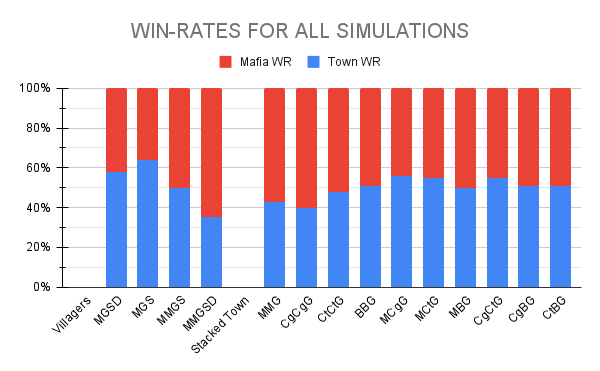
\includegraphics[width=1\linewidth]{figures/Winrates}
    \caption{\\Graph of the win-rate of various simulated game compositions.\\
        There were 10 players in each simulation.\\
        Each simulation was 100 games.
        Simulation names are related to team composition, based on role
        abbreviations in appendix \ref{app:A}.\\
        The first 4 runs labelled \textit{Villagers} means that all roles not
        mentioned in the abbreviation are replaced with villagers.\\
        The next runs labelled \textit{Powerful Town} means that all roles not
        mentioned in the abbreviation are replaced with	one of each town role.}
    \label{fig:VariousSimulations}
\end{figure}
\todo{Too much text in the caption}
\vspace{-5px}Based on this graph we can deduce that mafiosi and
consiglieri are more
impactful for the mafia than both consorts and blackmailers. But it also seems
that the varied team consisting of one mafioso, consigliere, and godfather,
performs marginally better than other mixed configurations. \\
The results indicate \todo{Refer to where this indicates this} that when playing against a powerful town, it is more
important for the mafia to be able to continually eliminate town members, and to be
able to quickly find the most powerful roles of the town, in order to eliminate
them, than it is to deny actions and communication to the town. \\
It would be interesting to see which of the non-eliminating mafia roles perform
best when they are on their own, and which composition of them performs best.
This type of game removes the mafias ability to eliminate during the night, while
they retain their knowledge of one another and their respective abilities to
gain information, limit nightly actions, and limit communicative actions. Figure \ref{fig:VariousSimulationsNonKilling} shows
are the results of such games:
\begin{figure}[H]
    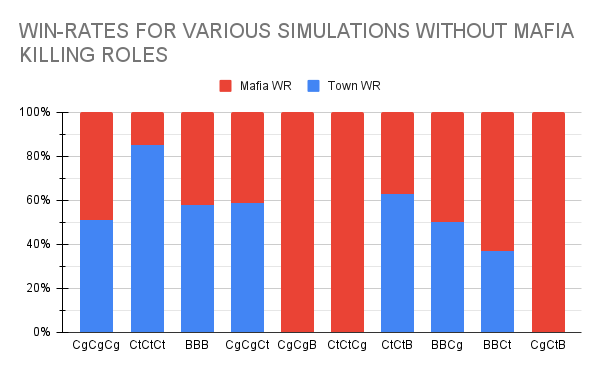
\includegraphics[width=1\linewidth]{figures/Winrates_NonKilling}
    \caption{\\Graph of the win-rate of various simulated game compositions
        with only non-eliminating mafia roles.\\
        There were 10 players in each simulation.\\
        Each simulation was 100 games.
        Simulation names are related to team composition, based on role
        abbreviations in appendix \ref{app:A}.\\
        All of the runs were against the previously explained powerful town.}
    \label{fig:VariousSimulationsNonKilling}
\end{figure}
\vspace{-5px} As seen on the above graph we can once again conclude that
consiglieri are more impactful than either consorts or blackmailers \ref{fig:VariousSimulationsNonKilling}. This may
be due to their superior abilities in finding the sheriff, enabling them to
collectively vote them out. It also seems that no mixed-combination of
non-killing mafia roles can compete with the pure-consiglieri team, except for BBCg.


\clearpage
\section{Appendix A}\label{app:A}
\begin{center}
	\textbf{Game Roles}
\end{center}
The following is a detailed description of the different roles and their unique
nightly actions:

\textbf{Roles allied to the town:}
\begin{enumerate}
	\item\textbf{Villager (V)} is a  role with no special actions. Typically
	      given
	      to the majority of the town.
	\item\textbf{Sheriff (S)} must choose one player each night and privately
	      gain
	      information regarding their faction.
	\item\textbf{Investigator (I)} must choose one player each night and
	      privately
	      gain information regarding a selection of roles that that player may have,
	      one of them being true.
	\item\textbf{Doctor (D)} must choose one player each night and protect them
	      from any harm that may come to them during the night.
	\item\textbf{Escort (E)} must choose one player each night and prevent them
	      from performing any actions during the night phase.
	\item\textbf{Veteran (Ve)} may choose to go on alert during the night
	      phase, if
	      they do so, then anyone targeting them at night will die.
	\item\textbf{Vigilante (Vi)} may choose to kill any one player during the
	      night
	      phase, if that player is revealed to be a member of the town during the
	      morning phase, the vigilante loses their killing ability, and will die the
	      following morning.
\end{enumerate}
\textbf{Roles allied to the mafia:}
\begin{enumerate}
	\item\textbf{Godfather (G)} must choose one player each night who will die.
	\item\textbf{Mafioso (M)} performs the killing on the Godfathers behalf. If
	      the
	      Godfather is targeted by an escort, then the Mafiosi may independently
	      choose who to kill. If the Mafiosi is targeted by the Escort, then the
	      Godfather kills their chosen target themselves.
	\item\textbf{Consigliere (Cg)} must choose one player each night and
	      privately
	      gain information regarding their role.
	\item\textbf{Consort (Ct)} must choose one player each night and prevent
	      them
	      from performing any actions during the night phase.
	\item\textbf{Framer (F)} must choose one player each night to frame. A
	      framed
	      player appears to be a member of the mafia if chosen by the Sheriff on this
	      night.
	\item\textbf{Blackmailer (B)} must choose one player each night to
	      blackmail. A
	      blackmailed player can only choose the “do not say anything” communicative
	      action.
\end{enumerate}
\section*{Appendix B}\label{app:B}
\begin{center}
	\textbf{Semantic Examples}
\end{center}
\textbf{(1)} \\
If one inquires another, the answer, gamma, could be of any of the 
following forms: "I believe that person 1 is a member of the mafia.", "I believe 
that person 1 is not a member of the mafia.", or "I believe that person 1 is a 
member of the mafia, and that person 2 is a member of the town."  \\ \\
\textbf{(2)} \\
No more oracle? \\ \\
\textbf{(3)} \\
This describes every individual agent's worldview. It consists of a 
non-empty set of possible worlds, in which some are epistemicly equivalent to 
each other. This is due to the agent's limited knowledge. These worlds contain facts, 
such as a person 1-2-3 being role x-y-z. Furthermore, agents implicitly know 
all inference rules, such as, "if no one was killed during the night, then both 
the mafioso and the godfather were targeted by escorts." Using this rule, an 
escort may be able to infer that, if that was the result of the night phase, 
then their target during the night is very likely to be one of those roles.  \\ 
\\
\textbf{(11), (12), (13)} \\
Simply states that a given agent can now update their worldview when a public announcement adds a new proposition to the common knowledge. The new worldview is a subset of the original worldview, in which 
all worlds where the proposition does not hold are excluded. 


~\cite{articletemplate}

\clearpage
% Bibliography
\printbibliography[heading=bibintoc, title=Bibliography]
\label{bib:mybiblio}

\end{document}
